\chapter{Qué comen los animales}\label{ch:g2:what-animals-eat}

El conejo del prado mordisquea hierba todo el día. Al zorro que cruza
ese mismo prado al atardecer la hierba no le interesa nada --- le
interesa el conejo. Y el mirlo toma lombrices por la mañana y cerezas
por la tarde. Todos los \omterm{def:g1:animals-around-us:animal}{animales} tienen que comer, pero no todos comen
lo mismo.

\section{Tres clases de comensales}

\begin{definition}[Herbívoro, carnívoro, omnívoro]\label{def:g2:what-animals-eat:kinds}
Los \omterm{def:g1:animals-around-us:animal}{animales} se clasifican según lo que comen:
\begin{itemize}
  \item un \emph{herbívoro}\index{herbívoro} come \omterm{def:g1:plants-around-us:plant}{plantas}: hierba,
        \omterm{def:g1:plants-around-us:parts}{hojas}, \omterm{def:g2:from-seed-to-plant:seed}{semillas}, fruta --- el conejo, la vaca, el caracol;
  \item un \emph{carnívoro}\index{carnívoro} come otros \omterm{def:g1:animals-around-us:animal}{animales}: el
        zorro, el gato, la mariquita (que caza pulgones diminutos);
  \item un \emph{omnívoro}\index{omnívoro} come \omterm{def:g1:plants-around-us:plant}{plantas} y \omterm{def:g1:animals-around-us:animal}{animales}:
        el mirlo, el jabalí --- y las personas.
\end{itemize}
\end{definition}

\begin{example}[Un prado, tres menús]\label{ex:g2:what-animals-eat:meadow}
En un prado de verano: el conejo corta la hierba (\omterm{def:g2:what-animals-eat:kinds}{herbívoro}); el zorro
caza al conejo (\omterm{def:g2:what-animals-eat:kinds}{carnívoro}); el mirlo toma una lombriz ahora y una
cereza después (\omterm{def:g2:what-animals-eat:kinds}{omnívoro}). Tres vecinos, tres menús --- y fíjate en que
la cena del zorro comió hierba antes.
\end{example}

\begin{omfigure}
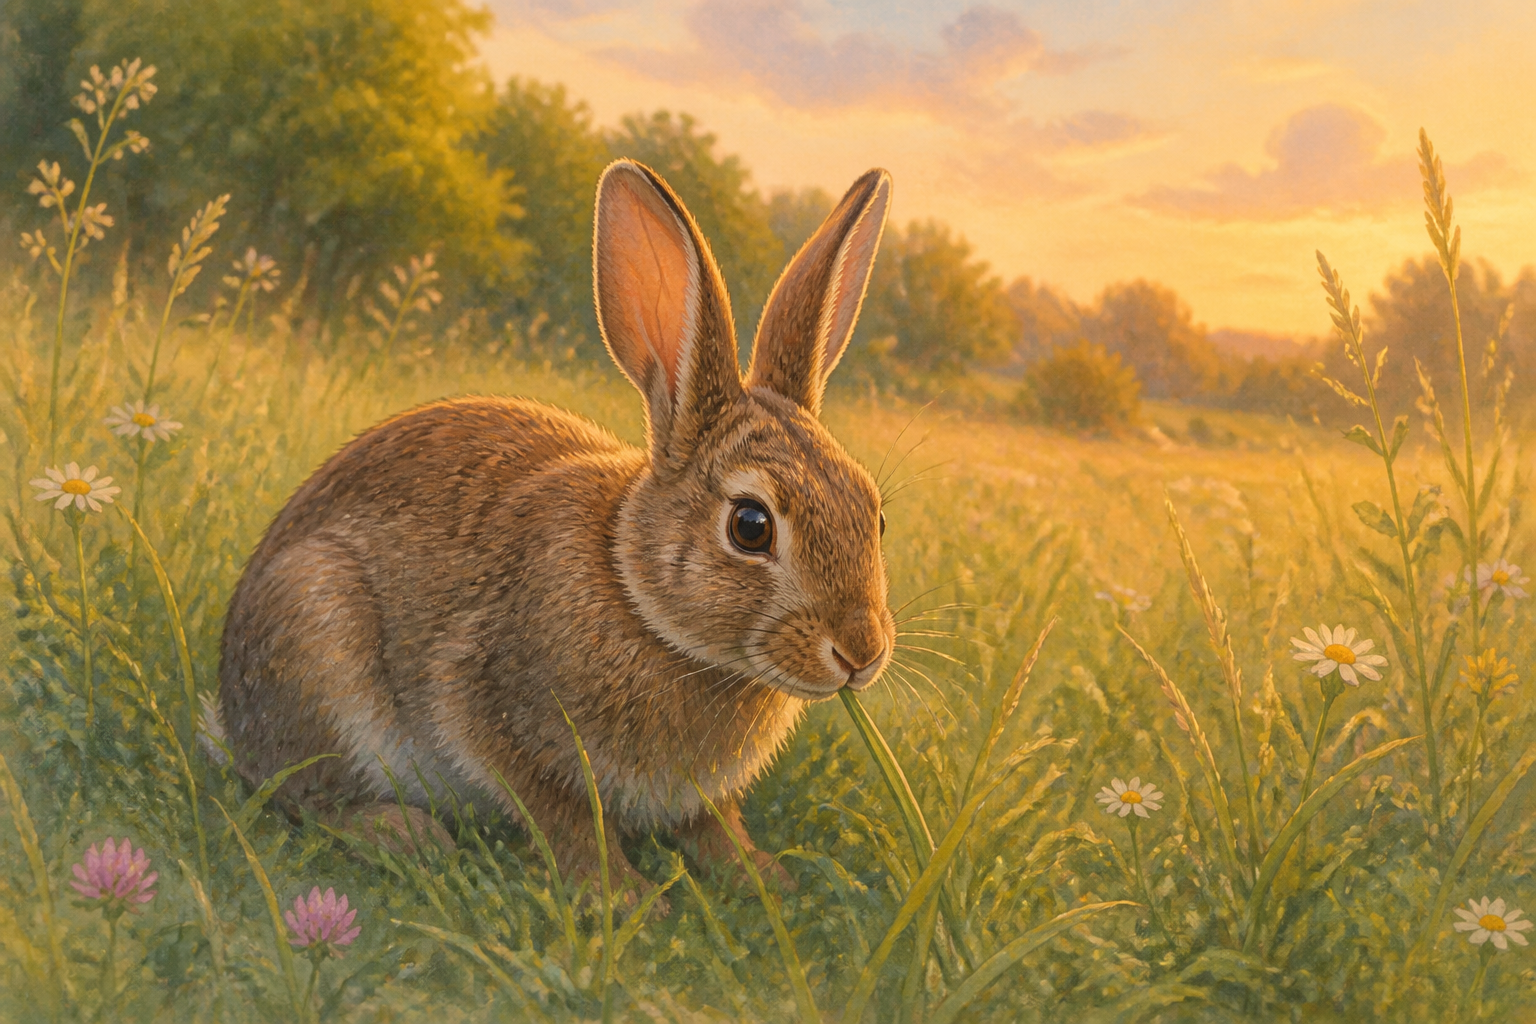
\includegraphics[width=0.6\linewidth]{images/book1/ai/g2-eat-rabbit.png}

{\small Un \omterm{def:g2:what-animals-eat:kinds}{herbívoro} en plena faena: el conejo y el prado, brizna a
brizna.}
\end{omfigure}

\begin{remark}[Los carnívoros no son los malos]\label{rem:g2:what-animals-eat:fox}
El zorro no es ``malo'' por comer conejos: cazar es sencillamente la
manera de alimentarse de un \omterm{def:g2:what-animals-eat:kinds}{carnívoro} --- tan natural como el
mordisqueo del conejo. En la naturaleza, comer y ser comido forman
parte del funcionamiento de la vida; un capítulo posterior enlazará
todas estas comidas en cadenas alimentarias.
\end{remark}

\section{Leer el menú de un animal en su cuerpo}

\begin{proposition}[El cuerpo va con el menú]\label{prop:g2:what-animals-eat:match}
El cuerpo de un \omterm{def:g1:animals-around-us:animal}{animal} lleva pistas sobre su comida:
\begin{itemize}
  \item los \omterm{def:g2:what-animals-eat:kinds}{herbívoros} como el conejo y la vaca tienen muelas grandes y
        planas para triturar \omterm{def:g1:plants-around-us:plant}{plantas}, y pasan muchas horas comiendo;
  \item los \omterm{def:g2:what-animals-eat:kinds}{carnívoros} como el gato y el zorro tienen dientes
        puntiagudos para agarrar a sus presas, garras afiladas y \omterm{def:g1:the-five-senses:sense}{ojos}
        mirando hacia delante para cazar;
  \item en las aves se ve en el pico: corto y grueso para cascar
        \omterm{def:g2:from-seed-to-plant:seed}{semillas} (el gorrión), curvo y ganchudo para desgarrar carne
        (el águila), largo y fino para sacar insectos de la corteza.
\end{itemize}
\end{proposition}
\admitted

\begin{omfigure}
\begin{minipage}[t]{0.31\linewidth}\centering
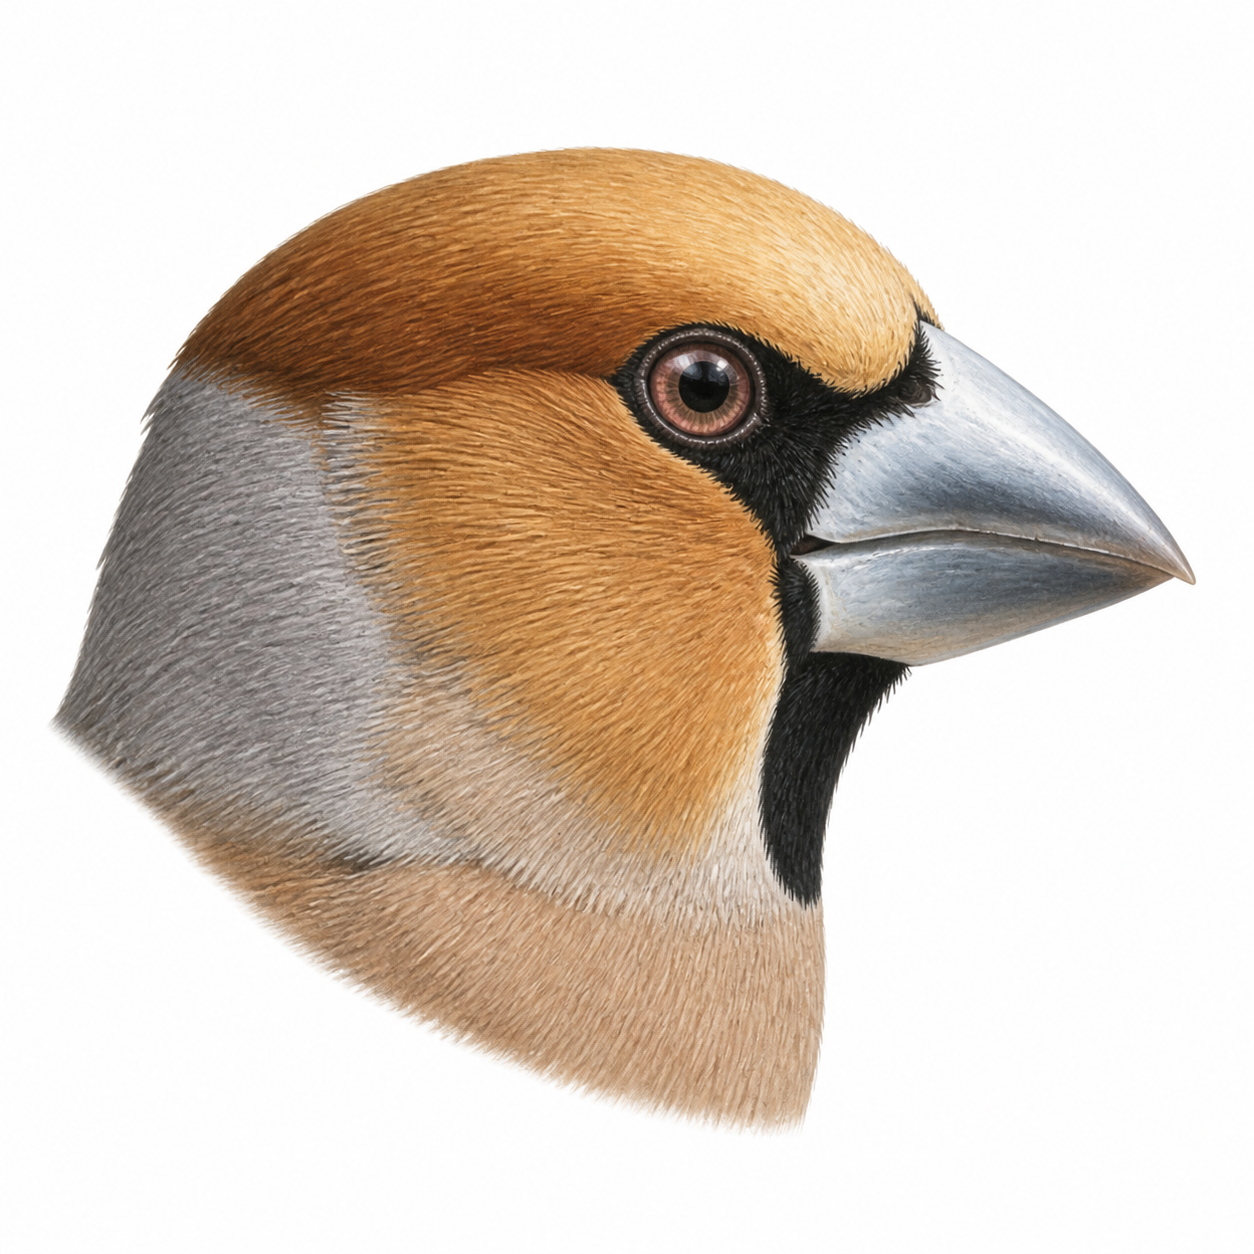
\includegraphics[width=\linewidth]{images/book1/ai/fig-beak-seed.png}

{\small pico corto y grueso:\\ casca \omterm{def:g2:from-seed-to-plant:seed}{semillas}}
\end{minipage}\hfill
\begin{minipage}[t]{0.31\linewidth}\centering
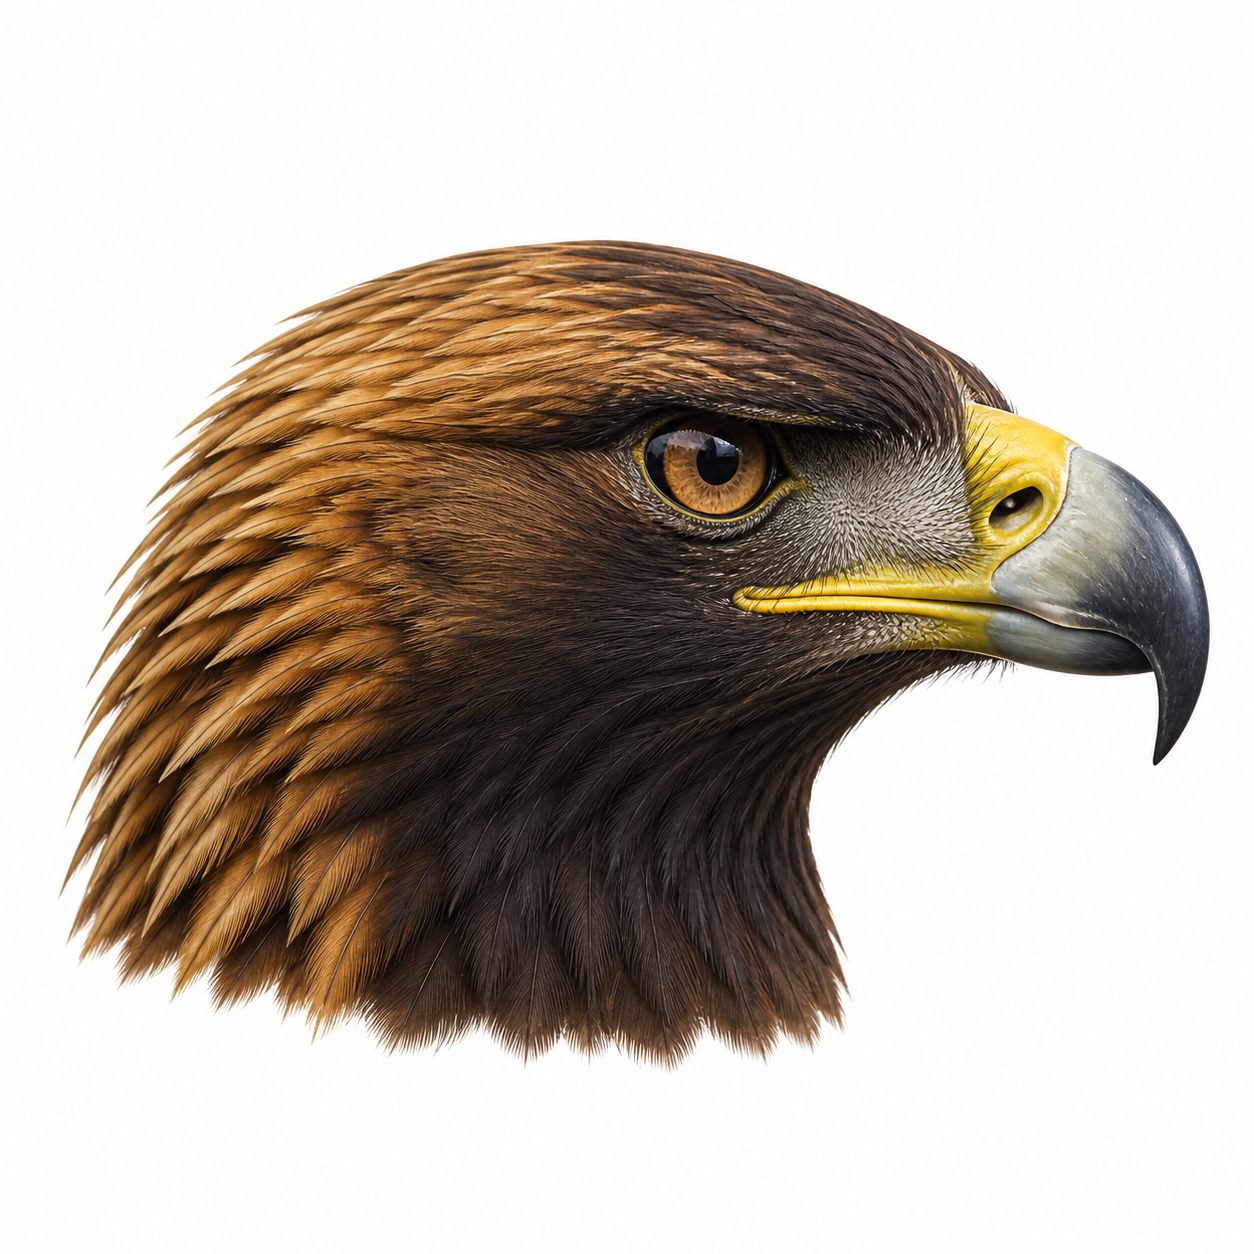
\includegraphics[width=\linewidth]{images/book1/ai/fig-beak-hook.png}

{\small pico ganchudo:\\ desgarra carne}
\end{minipage}\hfill
\begin{minipage}[t]{0.31\linewidth}\centering
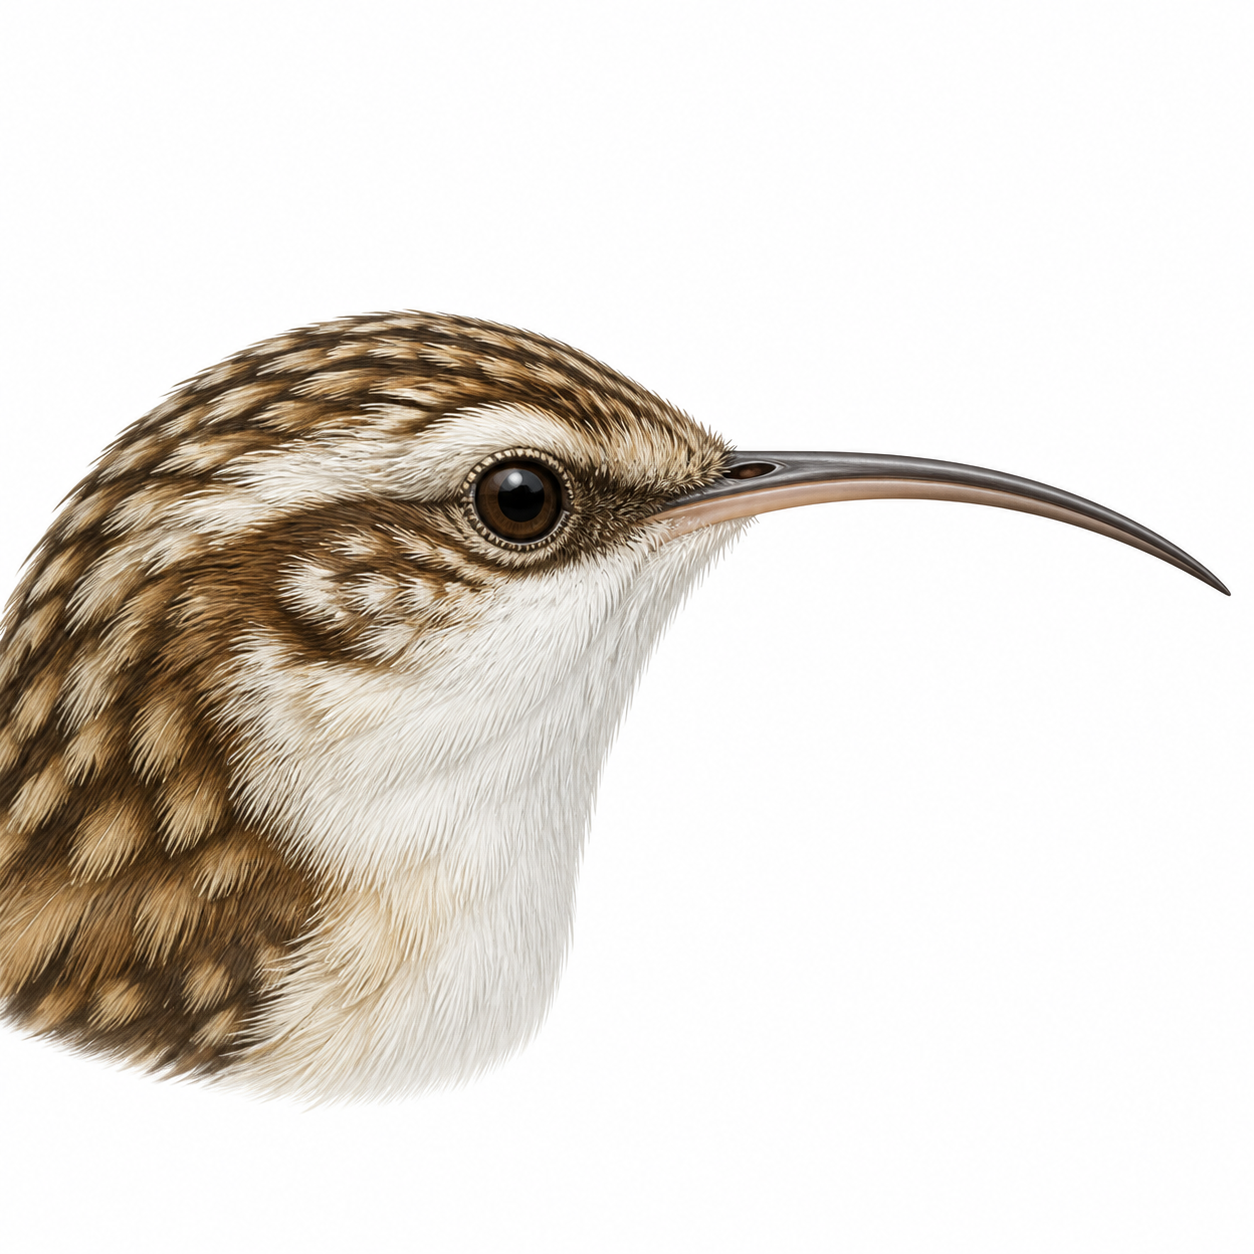
\includegraphics[width=\linewidth]{images/book1/ai/fig-beak-thin.png}

{\small pico largo y fino:\\ saca insectos}
\end{minipage}

\medskip
{\small Tres picos, tres menús: el pico de un ave es una herramienta
que su comida ha ido moldeando.}
\end{omfigure}

\begin{example}[Los dientes del gato]\label{ex:g2:what-animals-eat:cat}
Mira bostezar a un gato: dientes largos y puntiagudos en las esquinas
delanteras de la boca. Esos son dientes de agarrar --- el equipo de un
\omterm{def:g2:what-animals-eat:kinds}{carnívoro}. La vaca, al bostezar, no enseñaría ninguno: su boca es toda
muelas anchas y planas para la hierba.
\end{example}

\begin{method}[Adivinar un menú]\label{met:g2:what-animals-eat:guess}
Para adivinar qué come un \omterm{def:g1:animals-around-us:animal}{animal} desconocido:
\begin{enumerate}
  \item mírale los dientes o el pico: ¿muelas planas, dientes
        puntiagudos de agarrar, o las dos cosas?
  \item mírale las garras y los \omterm{def:g1:the-five-senses:sense}{ojos}: ¿son herramientas de caza o no?
  \item obsérvalo comer si puedes --- la pista más segura de todas;
  \item y después ponle nombre: \omterm{def:g2:what-animals-eat:kinds}{herbívoro}, \omterm{def:g2:what-animals-eat:kinds}{carnívoro} u \omterm{def:g2:what-animals-eat:kinds}{omnívoro}.
\end{enumerate}
\end{method}

\section{Comer bastante, día tras día}

\begin{proposition}[Alimentarse es una tarea diaria]\label{prop:g2:what-animals-eat:daily}
La comida es el combustible y el material de construcción del cuerpo,
así que los \omterm{def:g1:animals-around-us:animal}{animales} tienen que comer una y otra vez, día tras día.
Cuánto tiempo les cuesta depende del menú: la hierba da poco en cada
bocado, así que la vaca pasta durante horas; la carne alimenta mucho,
así que al zorro le puede bastar una buena comida y descansar.
\end{proposition}
\admitted

\begin{example}[El invierno cambia el menú]\label{ex:g2:what-animals-eat:winter}
La comida cambia con las estaciones. El mirlo come lombrices e
insectos en verano, pero en invierno, cuando el suelo está duro, se
pasa a las bayas. El menú amplio de un \omterm{def:g2:what-animals-eat:kinds}{omnívoro} es una gran ayuda
cuando vienen mal dadas.
\end{example}

\section{Ejercicios}

\begin{exercise}[$\star$]\label{exo:g2:what-animals-eat:1}
Di las palabras para: un \omterm{def:g1:animals-around-us:animal}{animal} que come \omterm{def:g1:plants-around-us:plant}{plantas}; un \omterm{def:g1:animals-around-us:animal}{animal} que come
otros \omterm{def:g1:animals-around-us:animal}{animales}; un \omterm{def:g1:animals-around-us:animal}{animal} que come de todo.
\end{exercise}

\begin{exercise}[$\star$]\label{exo:g2:what-animals-eat:2}
¿\omterm{def:g2:what-animals-eat:kinds}{Herbívoro}, \omterm{def:g2:what-animals-eat:kinds}{carnívoro} u \omterm{def:g2:what-animals-eat:kinds}{omnívoro}: (a) la vaca? (b) el zorro? (c) el
mirlo? (d) el caracol? (e) la persona?
\end{exercise}

\begin{exercise}[$\star$]\label{exo:g2:what-animals-eat:3}
¿Qué dientes necesita más un \omterm{def:g2:what-animals-eat:kinds}{herbívoro}: muelas planas o dientes
puntiagudos de agarrar? ¿Por qué?
\end{exercise}

\begin{exercise}[$\star$]\label{exo:g2:what-animals-eat:4}
Empareja cada pico con un menú: corto y grueso; curvo y ganchudo;
largo y fino.
\end{exercise}

\begin{exercise}[$\star$]\label{exo:g2:what-animals-eat:5}
La mariquita es pequeña, bonita --- y carnívora. ¿Qué caza?
\end{exercise}

\begin{exercise}[$\star$]\label{exo:g2:what-animals-eat:6}
¿Por qué pasa la vaca muchas más horas comiendo que el zorro? Usa la
\cref{prop:g2:what-animals-eat:daily}.
\end{exercise}

\begin{exercise}[$\star$]\label{exo:g2:what-animals-eat:7}
¿Qué come el mirlo en verano y qué come en invierno? ¿Por qué es útil
un menú amplio?
\end{exercise}

\begin{exercise}[$\star$]\label{exo:g2:what-animals-eat:8}
Pruébalo: observa a los pájaros en un parque o en un comedero. Anota
lo que coge cada especie --- \omterm{def:g2:from-seed-to-plant:seed}{semillas}, pan, insectos, bayas --- y
mírales el pico. ¿Se cumple la \cref{prop:g2:what-animals-eat:match}?
\end{exercise}

\begin{exercise}[$\star\star$]\label{exo:g2:what-animals-eat:9}
A un zoo le llega un \omterm{def:g1:animals-around-us:animal}{animal} misterioso: dientes delanteros
puntiagudos, garras afiladas, \omterm{def:g1:the-five-senses:sense}{ojos} mirando hacia delante. ¿Cuál es su
menú probable? ¿Qué pasos del \cref{met:g2:what-animals-eat:guess} has
usado?
\end{exercise}

\begin{exercise}[$\star\star$]\label{exo:g2:what-animals-eat:10}
``Sin hierba pronto no habría zorros''. El zorro no come hierba nunca
--- y, aun así, la frase es correcta. Explícalo con el prado del
\cref{ex:g2:what-animals-eat:meadow}.
\end{exercise}
